\documentclass[12pt]{article}

% Packages
\usepackage{graphicx} 
\usepackage{caption}
\usepackage{subcaption}
\usepackage{amsmath}
\usepackage{hyperref} 
\usepackage{geometry} 
\usepackage{float}
\geometry{a4paper, margin=1in} 
\usepackage{xcolor}
\hypersetup{
    colorlinks,
    linkcolor={red!50!black},
    citecolor={blue!50!black},
    urlcolor={blue!50!black}
}

% Load polyglossia package
\usepackage{polyglossia}

% Set up English and Greek as the languages
\setdefaultlanguage{greek}  % Set English as the default language
\setotherlanguage{english}      % Set Greek as an additional language

% Load fonts (for XeLaTeX or LuaLaTeX)
\newfontfamily\greekfont[Script=Greek]{GFS Didot}  % Greek font
\newfontfamily\greekfonttt[Script=Greek]{Inconsolata}  % Greek monospace font

\newcommand{\repo}{\href{https://github.com/Selivanof/university-collection/tree/main/RealTime_Embedded_Systems}{repo }}

\newcommand{\config}{\href{https://github.com/Selivanof/university-collection/tree/main/RealTime_Embedded_Systems/performance/websocket_config.json}{\texttt{websocket\_config.json} }}

\newcommand{\scripts}[1]{\href{https://github.com/Selivanof/university-collection/tree/main/RealTime_Embedded_Systems/scripts}{\texttt{#1}}}

% Title
\title{%
  Αναφορά Εργασίας \\[1em]
  \large Ενσωματωμένα Συστήματα Πραγματικού Χρόνου \\[2em]
  \textit{Εαρινό Εξάμηνο 2024} \vfill }
\author{Γεώργιος Σελιβάνωφ \\
  \texttt{selivanof@ece.auth.gr}}
\date{\today}

\begin{document}

% Title Page
\maketitle
\thispagestyle{empty}
\newpage


% Table of Contents
\tableofcontents
% Add your note here
\begin{center}
    \textbf{Σημείωση:}
    \textit{Έγινε η βέλτιστη δυνατή προσπάθεια να περιοριστεί το μέγεθος της αναφοράς στις ενδεδειγμένες 4 σελίδες, παρόλα αυτά το τελικό μέγεθος της είναι 6 σελίδες, ώστε τα γραφήματα και οι πίνακες να είναι μεγάλα και ευανάγνωστα. Πολλά σημεία της υλοποίησης αναφέρονται επιγραμματικά, καθώς έπρεπε επίσης να αναφερθούν - μεταξύ άλλων - προβλήματα του API, παραδοχές και υποθέσεις που έγιναν καθώς και ο τρόπος διασφάλισης της ορθής λριτουργίας του προγράμματος. Τα headers στο \repo της εργασίας περιέχουν αναλυτικές πληροφορίες σε θέματα υλοποίησης.}
\end{center}
\thispagestyle{empty}
\newpage
\setcounter{page}{1}
% Introduction
\section{Βασική Δομή Προγράμματος}
\subsection{Τεχνικές Πληροφορίες}
Για την υλοποίηση της εργασίας έγινε χρήση της γλώσσας C++. Χρησιμοποιήθηκαν οι βιλιοθήκες \href{https://libwebsockets.org/}{\textbf{libwebsockets}}, \href{https://simdjson.org/}{\textbf{simdjson}} και \href{https://fmt.dev/}{\textbf{fmt}}.

Όσον αφορά το cross-compiling, αναλυτική περιγραφή για τα βήματα που ακολουθήθηκαν υπάρχει στο \repo της εργασίας.

\subsection{Σημαντικές Παρατηρήσεις}
\label{subsec:notes}
Πριν αναλυθούν ορισμένες μέθοδοι που χρησιμοποιήθηκαν, ακολουθούν συνοπτικά ορισμένες παρατηρήσεις σχετικά με την λειτουργία της εφαρμογής:
\begin{itemize}
    \item Το API του Finnhub \textbf{δεν} στέλνει τα trades με αυστηρή χρονολιγική σειρά. Για αυτόν τον λόγο, στα πλαίσια της εφαρμογής θεωρήθηκε ότι τα trades που λαμβάνονται μπορεί να αφορούν \textbf{οποιαδήποτε} χρονική στιγμή.
    \item Προφανώς δεν γίνεται να ξέρουμε άμα έχουμε λάβει όλα τα μηνύματα που αφορούν το λεπτό που μόλις πέρασε, τόσο λόγο του παραπάνω όσο και των καθυστερήσεων του δικτύου. Τα ζητούμενα στατιστικά λεπτόυ υπολογίζονται με τα δεδομένα που έχουν ληφθεί μέχρι την χρονική στιγμή που τα γράφουμε στο αρχείο.
    \item Μηνμύματα που αφορούν σύμβολα \textbf{Forex} έχουν \href{https://github.com/finnhubio/Finnhub-API/issues/213}{μηδενικό volume} . Για τον υπολογισμό των στατιστικών, θεωρούνται όλα τα μηνύματα ισάξια με μοναδιαίο volume.
    \item Σε περίπτωση που στο τέλος του λεπτού ληφθούν trades με το ίδιο timestamp, closing price θεωρείται η τιμή αυτού που έπεται, θεωρώντας ότι το Finnhub έχει μεριμνήσει και τα τοποθετεί αναλόγως στο μήνυμα.
\end{itemize}

\subsection{Ροή των Trade}

Το κυρίως thread δέχεται και ερμηνεύει τα μηνύματα του Finnhub, αποτελώντας τον μοναδικό producer του προγράμματος. Από την πλευρά των consumer, εντοπίζουμε 2 διαφορετικά - ως προς την λειτουργία που πραγματοποιούν - είδη από workers πραγματικού χρόνου. Τους Recording Workers που καταγράφουν τα trades σε αρχεία και τους Statistics Workers που ενημερώνουν τα στατιστικά (κινούμενο μέσο όρο και candlestick).

Κάθε worker έχει το δικό του queue σύμφωνα με το μοντέλο Single Producer - Single Consumer (SP-SC) και είναι υπεύθυνο για συγκεκριμένα σύμβολα, τα οποία μοιράζονται ισάξια\footnote{Το κάθε thread αναλαμβάνει ίσο αριθμό από σύμβολα. Θεωρείται ότι η λίστα συμβόλων που παρέχεται στο \texttt{websocket\_config.json} περιέχει έγκυρα σύμβολα, ειδάλλως θα ληφθούν και τα άκυρα σύμβολλα υπόψιν στην κατανομή.} στην αρχή του προγράμματος. Αν και η τακτική SP-SC δεν εγγυάται τον ισομερή καταμερισμό του φόρτου στα διαθέσιμα threads, πλεονεκτεί έναντι του μοντέλου Single Producer - Multiple Consumers, που θα οδηγούσε πιο συχνά σε ανταγωνισμούς για τα mutex.

Μια τρίτη κατηγορία από workers αποτελούν οι Exporting Workers, οι οποίοι κάθε λεπτό (XX:XX:00) καταγράφουν τα - ήδη υπολογισμένα - στατιστικά στα κατάλληλα αρχεία. Όπως και πριν, έτσι και σε αυτήν την περίπτωση στον κάθε worker έχουν ανατεθεί συγκεκριμένα σύμβολα.

Ο αριθμός των thread που θα διατεθούν για κάθε τύπο worker είναι παραμετροποιήσημος στο runtime με την βοήθεια του αρχείου \texttt{websocket\_config.json}.

\section{Ανάλυση Προγράμματος}
\subsection{Υπολογισμός στατιστικών σε πραγματικό χρόνο}
Η υπολογισμός των στατιστικών σε πραγματικό χρόνο επιτρέπει την -ανά λεπτό- εξαγωγή των στατιστικών σε αρχεία με πολύ μικρή καθυστέρηση, αφού όλα τα απαραίτητα δεδομένα έχουν ήδη υπολογιστεί σε πραγματικό χρόνο.

Η βασική δυσκολία στην υλοποίηση των μηχανισμών υπολογισμού των στατιστικών ήταν η σποραδική παραλαβή καθυστερημένων trades που αναφέρθηκε στο \ref{subsec:notes}. Για να επιλυθεί, χρησιμοποιήθηκαν τα \textbf{hashed} \texttt{std::unordered\_map} που προσφέρει η C++. Χρησιμοποιώντας timestamps της μορφής HH:MM:00 ως κλειδιά, μπορούμε σε σταθερό χρόνο O(1) να ενημερώσουμε τα στατιστικά του σωστού λεπτού για κάθε ληφθέν trade, ανεξαρτήτως της καθυστέρησης με την οποία λήφθηκαν.

Η συγκεκριμένη υλοποίηση \textbf{δεν διορθώνει} στατιστικά που έχουν ήδη καταγραφεί σε αρχεία. Για να εφαρμοστεί κάτι τέτοιο, θα ήταν προτιμότερο να χρησιμοποιηθεί \href{https://www.sqlite.org/}{βάση δεδομένων} για την καταγραφή των δεδομένων, ώστε να ελαχιστοποιηθούν οι χρόνοι αναζήτησης και επεξεργασίας των ήδη αποθηκευμένων στατιστικών. 

\subsection{Διαχείριση αρχείων και εγγραφών}

Με διαφορά η μεγαλύτερη καθυστέρηση στις εγγραφές οφειλόταν στην διαδικασία της εγγραφής σε αρχεία. Για αυτό τον λόγο δόθηκε ιδιαίτερη βαρύτητα σε αυτό το κομμάτι, ώστε να μειωθεί το overhead της εγγραφής στο ελάχιστο δυνατό. Συγκεκριμένα:

\begin{itemize}
    \item Αντί να ανοίγουν και να κλείνουν τα αρχεία με κάθε εγγραφή ο client τα διατηρεί ανοιχτά \textbf{καθ'όλη} τη διάρκεια εκτέλεσης του προγράμματος. Αυτό προϋποθέτει ότι τα αρχεία \textbf{δεν θα διαγραφούν} από τον χρήστη στο διάστημα αυτό. Η ανάγνωση, όπως και η αντιγραφή των αρχείων δεν επηρεάζει το πρόγραμμα.
    \item Οι εγγραφές στα αρχεία είναι από προεπιλογή \textbf{buffered} τόσο στην C όσο και στην C++. Αυτό έρχεται σε αντίθεση με την απαίτηση της εργασίας για καταγραφή σε \textbf{πραγματικό χρόνο}. Στην εφαρμογή αυτή, χρησιμοποιήθηκαν \textbf{unbuffered} \texttt{std::ofstream} για τις εγγραφές, επιτυγχάνοντας εγγραφή σε πραγματικό χρόνο, βελτίωση της απόδοσης (σε σχέση με \texttt{fflush} μετά από κάθε εγγραφή), και μείωση της χρήσης μνήμης.
\end{itemize}

\subsection{Πρακτικές ελαχιστοποίησης καθυστερήσεων}
Επιγραμματικά αναφέρονται ορισμένες πρακτικές που ακολουθήθηκαν για να μειωθούν οι καθυστερήσεις στο ελάχιστο δυνατό:
\begin{itemize}
\setlength\itemsep{0em}
    \item Περιορισμός των \textbf{lock} στο ελάχιστο δυνατό \textbf{scope}, μειώνοντας τον αριθμό των εν δυνάμει ανταγωνισμών για τα mutex.
    \item Αποφυγή αχρείαστων αντιγραφών με την χρήση \textbf{references} και της \textbf{std::move}.
    \item Ορισμός \textbf{inline} συναρτήσεων για απλές επαναλαμβανόμενες διαδικασίες.
    \item Πλήρης \textbf{αποφυγή} χρήσης \textbf{virtual} μεθόδων/κλάσεων.
    \item Χρήση \textbf{templates} έναντι εναλλακτικών, όπου ήταν εφικτό.
    \item Δυνατότητα \textbf{δέσμευσης των threads} σε συγκεκριμένους πυρήνες της CPU, ανάλογα την την δουλεία που εκτελούν (μέσω του config).
\end{itemize}

\section{Μετρήσεις}
Η πραγματοποίηση των μετρήσεων έγινε με τον μέγιστο αριθμό συμβόλων που επιτρέπει το δωρέαν API του Finnhub (50). Αποτελούνται από τα 30 πιο ενεργά σύμβολα, 10 πιο ενεργά κρυπτονομίσματα και 10 πιο ενεργά συναλλάγματα\footnote{Πηγή: \href{https://finance.yahoo.com/markets}{Yahoo Finance}}. Χρησιμοποιήθηκε το \config που βρίσκεται στο repo της εργασίας (εγγραφή σε δημοφιλή σύμβολα). 

Αν και αρχικά οι μετρήσεις έγιναν σε ημέρες που λειτουργεί το χρηματιστήριο, παρατηρήθηκε πως είχε παραληφθεί η καταγραφή του όγκου στα στατιστικά. Αναγκαστικά, οι τελικές μετρήσεις έγιναν στις μόνες διαθέσιμες ημέρες (Παρασκευή - Σάββατο). Αν και τα 20 από τα 50 σύμβολα λειτουργούν και το Σάββατο, θεωρήθηκε σκόπιμο να χωριστούν όλες οι καθυστερήσεις σε 1ο και 2ο εικοσιτετράωρο, όπου το σύστημα λάμβανε -κατά κύριο λόγο - μηνύματα για 50 και 20 σύμβολα αντίστοιχα. Παρόλα αυτά, όπως φαίνεται και παρακάτω, δεν υπήρχαν διαφορές ανάμεσά τους.

\subsection{Καθυστερήσεις καταγραφών πραγματικού χρόνου}
Οι καθυστερήσεις για την εγγραφή σε πραγματικό χρόνο υπολογίζονται από την διαφορά το timestamp άφιξης των trades στο σύστημα και του timestamp ακριβώς πριν την εγγραφή\footnote{Αν και το δεύτερο timestamp δεν περιλαμβάνει τον χρόνο εκτέλεσης της εντολής \texttt{write}, αυτός αποτυπώνεται \textbf{εμμέσως} αφού καθυστερείται η καταγραφή των υπόλοιπων trade που βρίσκονται στην ουρά. Το παραπάνω επιβεβαιώθηκε καταγράφοντας σε ξεχωριστό 24ωρο τη μέση τιμή των καθυστερήσεων με το δεύτερο timestamp \textbf{μετά} την εντολή εγγραφής, αποθηκεύοντας την στη μνήμη μέχρι την έξοδο του προγράμματος.}. Για να βεβαιωθούμε ότι το timestamp άφιξης είναι όσο το δυνατόν πιο ακριβές:
\begin{itemize}
    \item Το timestamp άφιξης υπολογίζεται όσο το δυνατόν γρηγορότερα (πρώτη εντολή της callback άφιξης μηνύματος).
    \item Επιβεβαιώθηκε πως η μέγιστη διάρκεια της callback άφιξης μηνύματος  (avg: 104μs, \textbf{max: 598μs}) ήταν μικρότερη από το ελάχιστο μεσοδιάστημα λήψης μηνυμάτων από το websocket (avg: 73ms, \textbf{min: 3ms}).
        \item Δεσμεύτηκε ο Πυρήνας 0 της CPU για το κυρίως thread και την αποδοχή μηνυμάτων από το Finnhub.
\end{itemize}



\begin{table}[H]
    \centering
    \begin{tabular}{lcccc}
        \textbf{Στατιστικό} & \textbf{1ο 24ωρο} & \textbf{2ο 24ωρο} & \textbf{Όλο το 48ωρο}  \\
        \hline
        Μέση Τιμή     & 159.59 μs & 154.7 μs & 159.26 μs    \\
        Διάμεσος  & 137 μs & 146 μs & 138 μs \\
        1\% High & 409 μs & 376 μs & 405 μs  \\
        Μέγιστο      & 1590652 μs & 4838 μs & 1590652 μs \\
        Ελάχιστο      & 7 μs & 10 μs & 7 μs  \\
    \end{tabular}
    \caption{Στατιστικά Καθυστερήσεων εγγραφών πραγματικού χρόνου}
    \label{tab:minute_statistics}
\end{table}

\begin{figure}[H]
    \centering
    \begin{minipage}{0.8\textwidth}
        \centering
        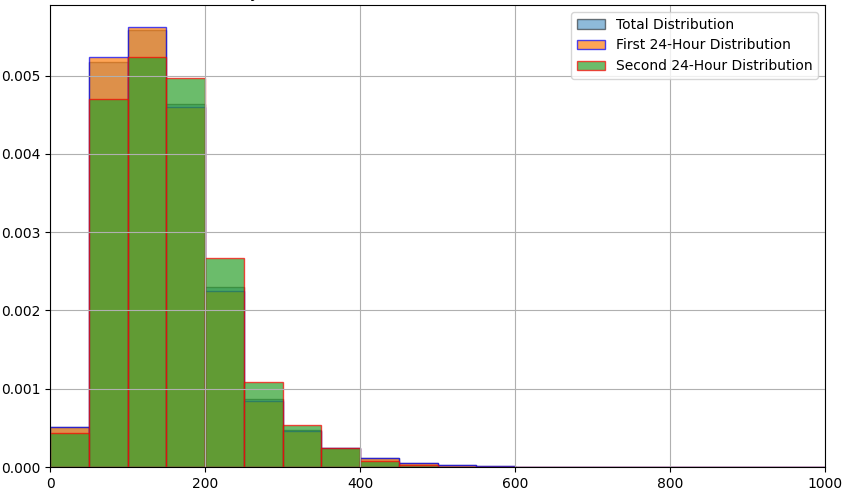
\includegraphics[width=\linewidth]{records.png} % First image
        \caption{Κατανομές των καθυστερήσεων}
        \label{fig:recs}
    \end{minipage}
\end{figure}


Η κατανομή των καθυστερήσεων προσεγγίζει την Log-Normal\footnote{Q-Q plot στο \scripts{recording\_delays.py}}, όπως ήταν αναμενόμενο καθώς οι παράγοντες που συμβάλλουν στην μεταβλητότητα των καθυστερήσεων (επιπλέον φόρτος συστήματος, χρόνος πρόσβασης SD κάρτας, κλπ) ακολουθούν Κανονική ή Log-Normal κατανομή. Η επικράτηση της Log-Normal έναντι της Κανονικής κατανομής οφείλεται στην ύπαρξη ενός ελάχιστου χρόνου κάτω από τον οποίο είναι πρακτικά αδύνατο να ερμηνευθεί και να καταγραφεί ένα trade.


\subsection{Καθυστερήσεις καταγραφών στατιστικών ανά λεπτό}
Οι καθυστερήσεις για τον υπολογισμό των στατιστικών ανά λεπτό υπολογίζονται από την διαφόρα του timestamp ΧΧ:ΧΧ:00 και του timestamp ακριβώς πριν την εγγραφή. Για να έχουν νόημα οι μετρήσεις, πρέπει να επιβεβαιώσουμε ότι ο υπολογισμός των στατιστικών σε πραγματικό χρόνο δεν καθυστερεί και άρα τα στατιστικά που καταγράφει ο exporting worker περιέχουν όλα τα trades \textbf{που έχουν ληφθεί στο σύστημα} μέχρι την χρονική στιγμή XX:XX:00. Για να επιβεβαιώσουμε τα παραπάνω:
\begin{itemize}
    \item Μετρήθηκε πως η μέση διάρκεια εκτέλεσης της \texttt{update\_statistics}, που καλείται σε κάθε trade αμέσως μόλις τοποθετηθεί στο queue, είναι μόλις 1,2μs, με το υψηλότερο 1\% στα 4,1μs. Δεδομένου ότι κάθε μήνυμα του finnhub έχει \textbf{το πολύ} 10 trades, ο μέσος χρόνος υπολογισμού των στατιστικών ανά μήνυμα είναι \textit{περίπου} 12μs.
\end{itemize}

\begin{table}[H]
    \centering
    \begin{tabular}{lcccc}
        \textbf{Στατιστικό} & \textbf{1ο 24ωρο} & \textbf{2ο 24ωρο} & \textbf{Όλο το 48ωρο}  \\
        \hline
        Μέση Τιμή     & 619.1 μs & 574.88 μs & 595.96 μs    \\
        Διάμεσος  & 631 μs & 587 μs & 608 μs \\
        1\% High & 1180 μs & 1129 μs & 1160 μs  \\
        Μέγιστο      & 1402 μs & 3264 μs & 3264 μs \\
        Ελάχιστο      & 63 μs & 71 μs & 63 μs  \\
    \end{tabular}
    \caption{Στατιστικά Καθυστερήσεων εγγραφών πραγματικού χρόνου}
    \label{tab:realtime_stats}
\end{table}

\begin{figure}[H]
    \centering
    \begin{minipage}{0.8\textwidth}
        \centering
        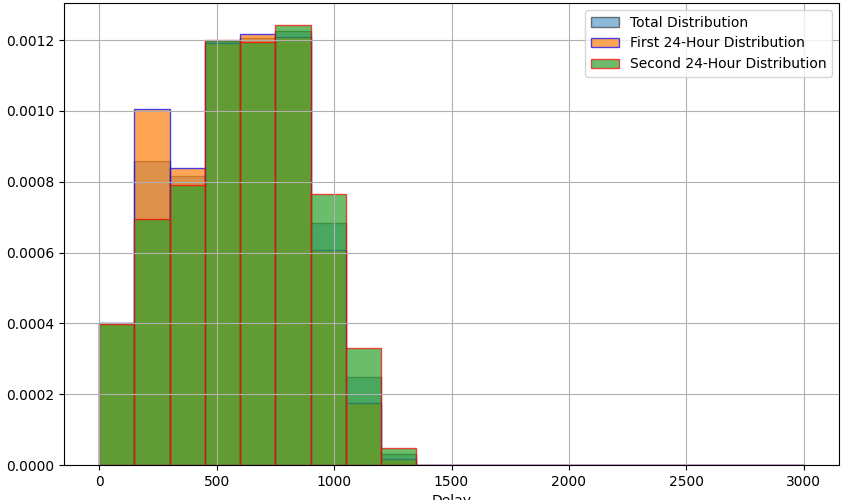
\includegraphics[width=\linewidth]{statistics.png} % First image
        \caption{Κατανομές των καθυστερήσεων}
        \label{fig:stats}
    \end{minipage}
\end{figure}

\subsection{Χρήση CPU}

Για τον υπολογισμό του ποσοστού που η CPU έμεινε αδρανής, χρησιμοποιήθηκε η συνάρτηση \texttt{getrusage}, η οποία επιστρέφει τον συνολικό χρόνο CPU που χρησιμοποίησε η διεργασία. Το κανονικοποιημένο, ως προς τους πυρήνες του Raspberry Pi, ποσοστό που μετρήθηκε ήταν \textbf{0.15\%}, χρησιμοποιώντας τον τύπο:

\[
    \text{Ποσοστό Χρήσης CPU} = \frac{\text{Χρόνος CPU}}{\text{Συνολικός Χρόνος Εκτέλεσης} \times \text{Φυσικοί Πυρήνες}}
\]
\section{Μακροχρόνια λειτουργία}
\subsection{Memory Profiling}
\begin{figure}[H]
    \centering
    \begin{minipage}{0.45\textwidth}
        Ένας πιθανός κίνδυνος για την μακροχρόνια λειτουργία του προγράμματος είναι τυχόν memory leaks που μπορεί να υπάρχουν στον κώδικα. 
        Για αυτόν τον λόγο, πραγματοποιήθηκε ένα 24ωρο memory profiling με την χρήση Valgrind (Massif), όπου δεν παρατηρήθηκαν σχετικά προβλήματα.
    \end{minipage}
    \hfill
    \begin{minipage}{0.45\textwidth}
        \centering
        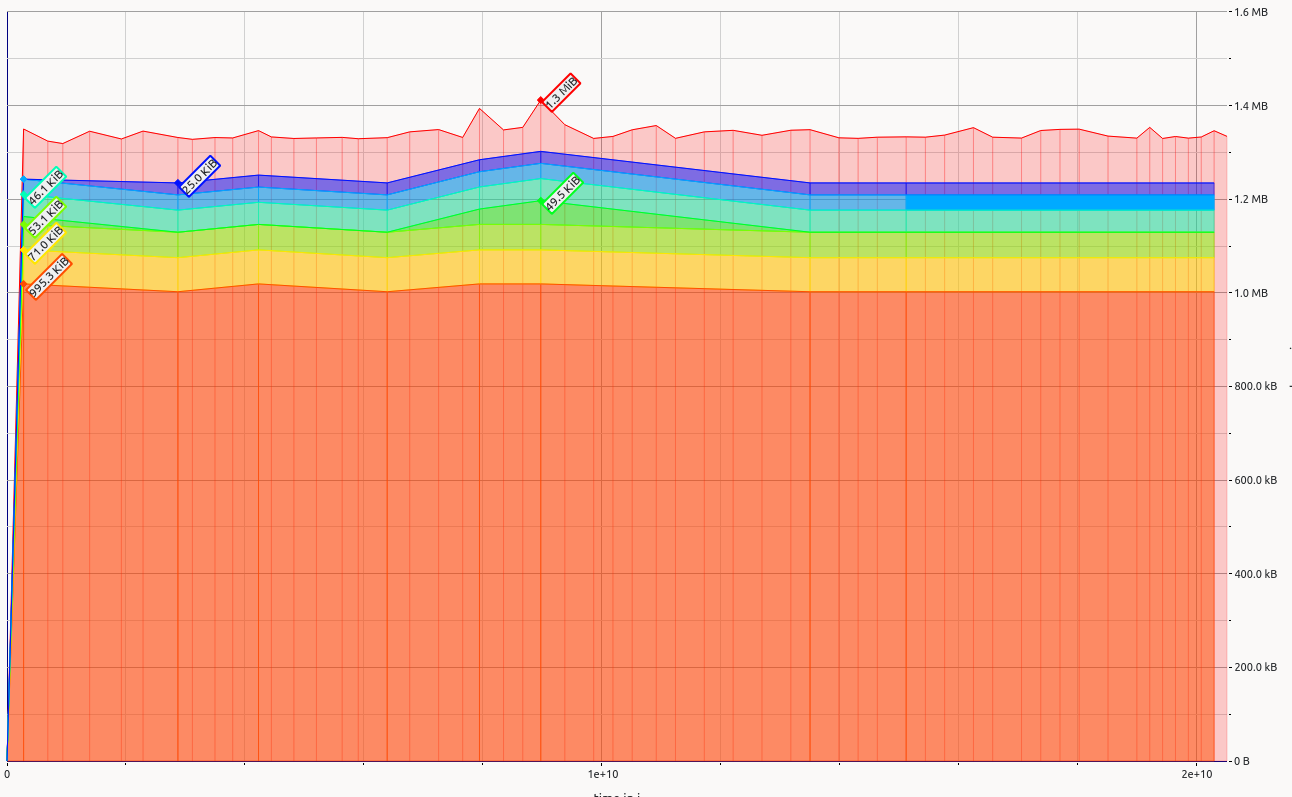
\includegraphics[width=\linewidth]{massif.png} % Use PNG format here
        \caption{Γράφημα δέσμευσης μνήμης για 24 ώρες λειτουργίας}
        \label{fig:massif}
    \end{minipage}
\end{figure}


\subsection{Διακοπές Δικτύου}
Για την αντιμετώπιση τυχών διακοπών του δικτύου, χρησιμοποιήθηκε ο υπάρχων μηχανισμός αποστολής μηνυμάτων ping σε αδρανείς συνδέσεις της libwebsockets σε συνδυασμό με το αντίστοιχο timeout. Σε περίπτωση μη επιθυμητής αποσύνδεσης, το σύστημα επανασυνδέεται στο Finnhub (με χρήση εκθετικών καθυστερήσεων). Παράλληλα διατηρεί ένα connection.log με όλες τις συνδέσεις και αποσυνδέσεις συνοδευόμενες από timestamp. Όλες οι σχετικές παράμετροι δύναται να ρυθμιστούν από τον χρήστη μέσω του \texttt{websocket\_config.json}.

\subsection{Πράξεις αριθμών κινητής υποδιαστολής}
Για τον υπολογισμό του κινούμενου μέσου όρου, καθώς και του όγκου ανά λεπτό, χρησιμοποιήθηκαν αθροίσματα αριθμών κινητής υποδιαστολής. Η αναπαράσταση τέτοιων αριθμών εμπεριέχει ένα σφάλμα το οποίο αν και μικρό, μπορεί μακροχρόνια να συσσωρευτεί και να οδηγήσει σε λανθασμένα αποτελέσματα. Για να αποφευχθεί αυτό, δεδομένου ότι το Finnhub έχει μέγιστη ακρίβεια 6 δεκαδικών ψηφίων\footnote{Αν και το API του Finnhub δεν διευκρινίζει το είδος των μεταβλητών που επιστρέφει, μετρήθηκε πειραματικά πως τα πεδία price και volume των μηνυμάτων δεν ξεπερνούσαν ποτέ τα 6 δεκαδικά ψηφία.}, όλα τα αθροίσματα αριθμών κινητής υποδιαστολής υλοποιήθηκαν μέσω \texttt{int64\_t}, πολλαπλασιάζοντας και διαιρώντας τους αριθμούς με 10\(^6\).
\end{document}
